\documentclass{article}
\usepackage{graphicx}

\graphicspath{{./img/}}
\title{2411 HW 4}
\author{Duncan Wilkie}
\date{1 October 2021}

\begin{document}

\maketitle

\section{}
The program appears in the Script Files section. The resulting plot of its output is immediately below.
\[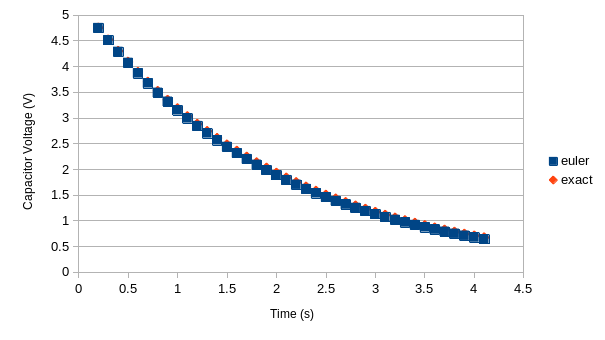
\includegraphics[scale=0.5]{plot1.png}\]
This shows quite good agreement between the exact result and Euler's algorithm, with a small accumulating undershoot in the computed values.

\section{}
\[\frac{dy}{dx}\bigg|_{x_0} = \frac{y(t_{n+1})-y(t_n)}{h}-O\left(\frac{h}{2}\frac{d^2y}{dx^2}\bigg|_{x_0}\right)=f(t,y)\]
\[\Rightarrow y_{n+1}=y+hf(t,y) + hO\left(\frac{h}{2}\frac{d^2y}{dx^2}\bigg|_{x_0}\right)\]
\[\Leftrightarrow y+hf(t,y) + O\left(\frac{h^2}{2}\frac{d^2y}{dx^2}\bigg|_{x_0}\right)\]
The absolute approximation error is this rightmost summand.

\section{}
We perform one Euler step to find $\frac{dx}{dt}$ at $t=0.2$:
\[\frac{dx}{dt}\bigg|_{0.2}=\frac{dx}{dt}\bigg|_{0}+(0.2)h=50.04\]
This enables us to perform the Euler step to find $x$:
\[x(0.2)=x(0)+(0.2)(50.04)=20.008\]


\end{document}
%%% Local Variables:
%%% mode: latex
%%% TeX-master: t
%%% End:
